%-----------------------------------------------------------------------------%
\chapter{\babTiga}
%-----------------------------------------------------------------------------%

%-----------------------------------------------------------------------------%
\section{NPACI Rocks}
%-----------------------------------------------------------------------------%

%-----------------------------------------------------------------------------%
\subsection{XZXX}
%-----------------------------------------------------------------------------%
Ini dapat dilihat di Gambar \ref{fig:alurkickstart} \citep{paper.jackson}. 

\begin{figure}
	\centering
	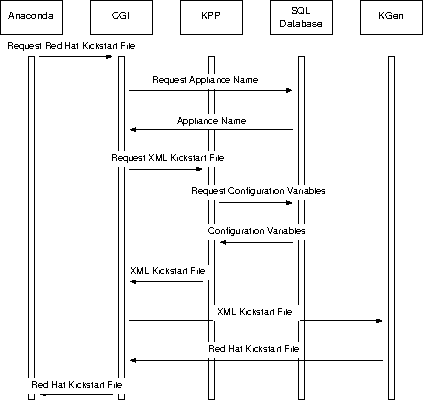
\includegraphics[width=0.8\textwidth,height=0.7\textwidth]
		{pics/alurkickstart.pdf}
	\caption{Alur Perjalanan \f{Kickstart}}
	\label{fig:alurkickstart}
\end{figure}
\begin{center}
{\small Sumber gambar: \citep{paper.jackson}}
\end{center}

Kata-kata dalam gambarnya bisa di hover, magic!!

%-----------------------------------------------------------------------------%
\subsection{Rocks Rolls}
%-----------------------------------------------------------------------------%
Untuk contoh konten Rolls dapat dilihat pada gambar \ref{fig:contohisiroll}. Pada contoh tersebut, \f{package} yang mengandung konfigurasi \f{graph} adalah berkas \co{roll-sge-kickstart-3.2.0-0.noarch.rpm} \citep{paper.jackson}. 


\begin{figure}
	\centering
	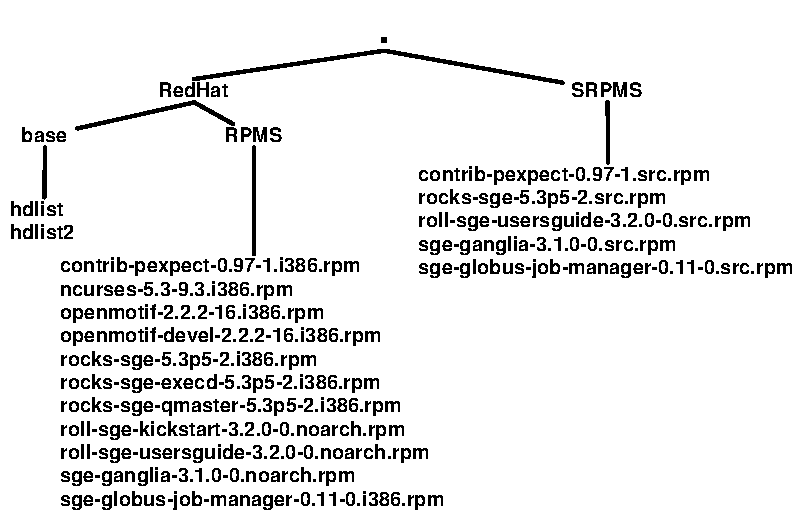
\includegraphics[width=0.9\textwidth,height=0.6\textwidth]
		{pics/rollexample.pdf}
	\caption{Contoh konten yang berada dalam \f{Rolls}}
	\label{fig:contohisiroll}
\end{figure}
\begin{center}
{\small Sumber gambar: \citep{paper.jackson}}
\end{center}

COde-like words : \code{FIRSTFIT} atau \code{BESTFIT} \citep{paper.jackson}. 

%-----------------------------------------------------------------------------%
\section{Mengubah Tampilan Teks}
%-----------------------------------------------------------------------------%
Beberapa perintah yang dapat digunakan untuk mengubah tampilan adalah: 
\begin{itemize}
	\item \bslash f \\
		Merupakan alias untuk perintah \bslash textit, contoh 
		\f{contoh hasil tulisan}.
	\item \bslash bi \\
		\bi{Contoh hasil tulisan}.
	\item \bslash bo \\
		\bo{Contoh hasil tulisan}.
	\item \bslash code \\ 
		\code{Contoh hasil tulisan}.
\end{itemize}


%-----------------------------------------------------------------------------%
\section{Memberikan Catatan}
%-----------------------------------------------------------------------------%
Ada dua perintah untuk memberikan catatan penulisan dalam dokumen yang Anda 
kerjakan, yaitu: 
\begin{itemize}
	\item \bslash todo \\
		Contoh: \\ \todo{Contoh bentuk todo.}
	\item \bslash todoCite \\ 
		Contoh: \todoCite
\end{itemize}


%-----------------------------------------------------------------------------%
\section{Menambah Isi Daftar Isi}
%-----------------------------------------------------------------------------%
Terkadang ada kebutuhan untuk memasukan kata-kata tertentu kedalam Daftar Isi. 
Perintah \bslash addChapter dapat digunakan untuk judul bab dalam Daftar isi. 
Contohnya dapat dilihat pada berkas thesis.tex.